\chapter{Funktionale Anforderungen}

    In diesem Abschnitt werden einzelne Funktionen des Workflows-System genauer vorgestellt.
    Anforderungen, die die Wunschkriterien beschreiben (nicht zwingend implementiert werden müssen) sind mit einem Stern (*) gekennzeichnet.
    
    \section{Anmeldung} \label{anmeldung:1}
        Um die folgenden Funktionen nutzen zu können, ist eine Anmeldung erforderlich.
    
    \section{Erstellung von Workflows\iffalse (Designers Interface)\fi} % just outcommented to make logo fit in header
        \begin{enumerate}[font={\bfseries}, label={FA\arabic*}0, wide=0pt, labelindent=1em, leftmargin=*]
        
            \item \label{workflowAnlegen:1} Einen neuen Workflow anlegen\newline
            Mit Hilfe des „New“ Buttons kann ein neuer Workflow mit Hilfe des graphischen Workflow Editors erstellt werden. Jeder Workflow hat einen Namen und eine Beschreibung.
            
                \subsection{Workflow Editor}
                Workflows sind als gerichtete azyklische Graphen (DAG) dargestellt. Das macht die Konstruktion einfach und übersichtlich. Einzelne Aufgaben eines Workflows werden durch die Knoten des Graphen und die Beziehungen zwischen verschiedenen Aufgaben durch die Kanten repräsentiert.
            
            \item \label{taskHinzufuegen:1} Task hinzufügen \newline
            Das Hinfügen der Knoten auf die Arbeitsoberfläche erfolgt mit Hilfe der \Gls{Drag and Drop}-Methode, was die Konstruktion des Workflow-Graphen intuitiv macht. In einer Toolbox auf der Seite befinden sich vorgegebene Knotenarten, die man zu dem Graphen hinzufügen kann. Nachdem man den Knoten positioniert hat, kann man die Aufgabe benennen.
        
            \item  \label{taskBearbeiten:1} Task bearbeiten \newline
            Die hinzugefügten Aufgaben auf der Arbeitsfläche können jederzeit bearbeitet werden. Eine Änderung des Namens einer Aufgabe kann durch Klicken auf diesen erfolgen. Die Position der Knoten kann ebenfalls jederzeit verändert werden.
            
            \item \label{taskLoeschen:1} Task löschen \newline
            Versehentlich hinzugefügte oder nicht mehr benötigte Aufgaben können per Klick gelöscht werden.
            
            \item  \label{kVerbinden:1} Knoten mit den Kanten verbinden \newline
            Um die Zusammenhänge zwischen zwei Aufgaben darzustellen, verbindet man zwei Knoten durch eine gerichtete Kante. Dabei kann die Aufgabe, auf die der Pfeil zeigt, nicht angefangen werden, solange die Aufgabe von der diese Kante ausgeht nicht erledigt wurde. \newline
            Man unterscheidet zwischen einem sequentiellen und einem parallelen Ablauf des Workflows.\newline
            Sequentiell bedeutet, dass Aufgaben nur in einer vorgegebenen Reihenfolge nacheinander ausgeführt werden können. Wenn es Aufgaben gibt, die voneinander unabhängig und gleichzeitig von mehreren Arbeitern gemacht werden können, spricht man über den parallelen Ablauf \newline
            
            Anhand eines kurzen Beispiels auf Abbildung \textbf{\ref{fig:seqpar}} wird der Unterschied klar. \newline
            Links ist die sequentielle, rechts die parallele Ausführung des selben Workflows abgebildet:
            
            \vspace{1.5cm}
            
            \begin{figure}[h]
                \centering
                \hspace*{-1.7cm}
                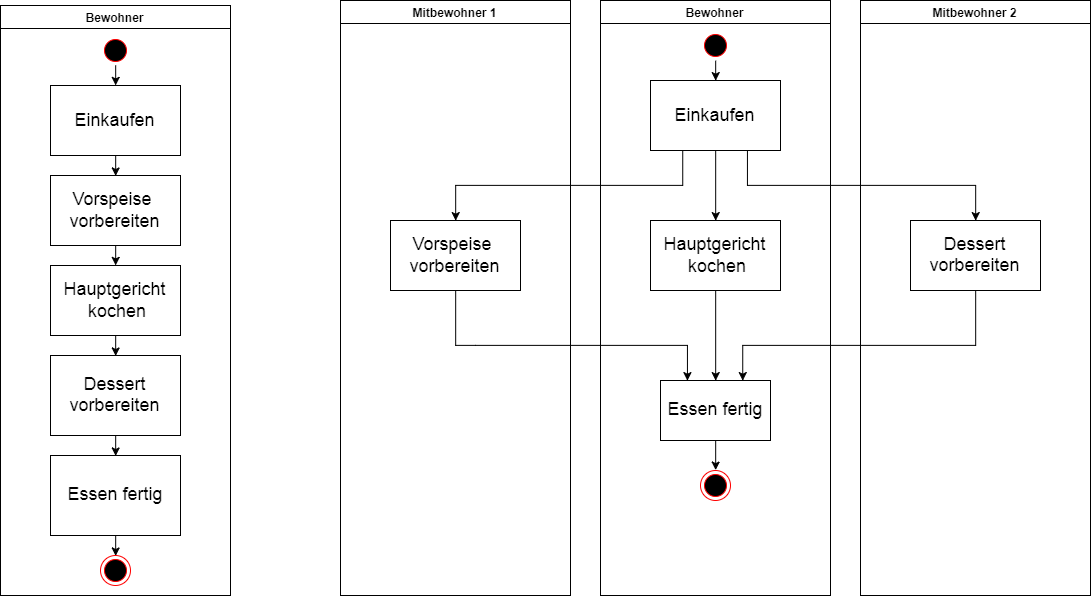
\includegraphics[width=18cm]{images/SequentiellParallelBeispiel.png}
                \caption{Sequentielle vs. parallele Ausführung des selben Workflows}
                \label{fig:seqpar}
            \end{figure}
            
            \item *Undo Funktion \newline
            In einer History werden alle Aktionen gespeichert und per Klick auf den „Undo“ Button (oder per Tastenkombination) kann die letzte Aktion mehrmals abgebrochen werden.
            
            \item  \label{interaktiveUnterstuetzung:1} Interaktive Unterstützung (Fehlermanagement)\newline
            Die gesamten Workflows und einzelnen Aufgaben werden in Echtzeit auf Syntax und Kompatibilität überprüft, was nur sinnvolle Kantenverbindungen zulässt. Falls bestimmte Regeln verletzt sind (zum Beispiel enthält der Graph einen Zyklus), wird eine Fehlermeldung auftauchen, in der der Grund für den Fehler und mögliche Lösungsansätze genau beschrieben sind.
            
            \item  \label{Sitzungswiederherstellung:1} Sitzungswiederherstellung \newline
            Für jeden Nutzer wird die letzte Sitzung gespeichert.\newline
            Falls vorhanden, kann der Nutzer seine letzte Sitzung nach dem Login wiederherstellen.
            
            \item \label{workflowImExport:1} *Workflow importieren/exportieren \newline 
            
            \item \label{workflowSpeichern:1} Workflow speichern \newline
             Gerade erstellte Workflows werden per Klick auf den „Save“ Button an den Server geschickt, der den Workflow in der Datenbank speichert. Nachdem man den Workflow gespeichert hat, wird er in der Liste angezeigt.
             
            \item  \iffalse \label{workflowSpeichern:1} \fi *Autosave Funktion \newline
            Anstatt manuell nach der Erstellung eines Workflow auf den „Save“ Button zu klicken, wird dieser automatisch alle 10-15 Sekunden in der Datenbank aktualisiert.
            
            \item \label{workflowAusfuehren:1} Workflow ausführen \newline
            Nachdem der Workflow erstellt und gespeichert wurde, kann man den mithilfe des „Run“ Buttons ausführen lassen.\
            
            \vspace{5cm}
            %\newpage
            
        \end{enumerate} % end enumeration and resume afterwards
        
        \section{Überwachung von Workflows}
        
        \begin{enumerate}[font={\bfseries}, label={FA\arabic*}0, wide=0pt, labelindent=1em, leftmargin=*, resume]
            
            \item  \label{workflowAuflisten:1} Workflows auflisten (Dashboard)\newline
            Auf der Workflows Seite werden alle gespeicherte Workflows mit dem Namen, Erstellungsdatum, Aktualisierungsdatum und Ausführungsstatus aufgelistet.
            
            \item  \label{workflowWiederherstellen:1} Workflow anzeigen \newline
            Mit dem Klick auf den Workflow in der Liste, wird der Workflowgraph angezeigt.
            
            \item  \label{workflowBearbeiten:1} Workflow bearbeiten \newline
            Den angezeigten Workflow kann man per Klick auf den „Edit“ Button im Editor bearbeiten. Neue Tasks kann man dynamisch in den existierenden Workflow einbinden.
            
            \item \label{workflowAbbrechen:1} Workflow abbrechen \newline
            Der gestartete Workflow kann jederzeit abgebrochen werden.
            
            \item  \label{workflowLoeschen:1} Workflow löschen \newline
            Abgebrochene oder noch nicht gestartete Workflows können gelöscht werden.
            
        \end{enumerate}
        
    \section{Systemfunktionen}
        \begin{itemize}
            \item Das Portal soll möglichst unabhängig vom Betriebssystem des Benutzers laufen\newline
                Wenn der Benutzer also:
                \begin{itemize}
                    \item Ein Browserprogramm installiert hat
                    \item Eine nicht zu alte Java-Version installiert hat
                    \item JavaScript im Browser erlaubt hat,
                \end{itemize}
                soll die Anwendung ohne Probleme laufen
        \end{itemize}
        
        
